% =========================================================
\chapter{Cálculo de los tiempos de arribo en la celda}
\label{ap:tiempos_arribo}
% =========================================================

La \cref{tab:tiempos_celda} reporta los tiempos de arribo al hidrófono
de la señal fotoacústica directa y de sus primeras reflexiones en las
fronteras de la celda. Este apéndice desarrolla el cálculo que la
sustenta y establece el procedimiento para recalcularla cuando la
geometría del montaje difiere de la nominal.

\begin{figure}[H]
  \centering
  \begin{subfigure}[b]{0.48\textwidth}
    \centering
    
\includegraphics[width=\textwidth]{base}
    \caption{Base (pieza 1).}
    \label{fig:plano_base}
  \end{subfigure}
  \hfill
  \begin{subfigure}[b]{0.48\textwidth}
    \centering
    
\includegraphics[width=\textwidth]{pared_laser_entrada}
    \caption{Pared larga con la ranura de la ventana de cuarzo (pieza 2).}
    \label{fig:plano_pared_laser}
  \end{subfigure}

  \vspace{1em}

  \begin{subfigure}[b]{0.32\textwidth}
    \centering
    
\includegraphics[width=\textwidth]{pared_hidrofono}
    \caption{Cabezal, \diameter\SI{12}{\milli\meter} (pieza 3).}
    \label{fig:plano_pared_h1}
  \end{subfigure}
  \hfill
  \begin{subfigure}[b]{0.32\textwidth}
    \centering
    
\includegraphics[width=\textwidth]{pared_hidrofono_2}
    \caption{Cuerpo, \diameter\SI{16}{\milli\meter} (pieza 4).}
    \label{fig:plano_pared_h2}
  \end{subfigure}
  \hfill
  \begin{subfigure}[b]{0.32\textwidth}
    \centering
    
\includegraphics[width=\textwidth]{pared_hidrofono_3}
    \caption{Cable, \diameter\SI{24}{\milli\meter} (pieza 5).}
    \label{fig:plano_pared_h3}
  \end{subfigure}

  \caption{Planos de fabricación de la celda fotoacústica, en acrílico de
           \SI{3}{\milli\meter} de espesor y con cotas en milímetros. Las
           tres placas de la pared del hidrófono son coaxiales y sus
           barrenos alojan sucesivamente el cabezal, el cuerpo y el cable
           del transductor, de modo que su eje se mantenga perpendicular
           al del haz. Tomados de Rangel Mendieta \cite{Rangel2023}.}
  \label{fig:planos_celda}
\end{figure}

\section*{Hipótesis geométricas}

El cálculo descansa en cuatro suposiciones, todas ellas consecuencia de
la construcción de la celda descrita en la \cref{sec:celda}.

La primera es que la región iluminada se comporta como una fuente
lineal. El haz atraviesa la cavidad a lo largo de su ancho interno,
aproximadamente \SI{70}{\milli\meter} según la \cref{fig:planos_celda},
con un diámetro mucho menor, de
modo que la columna de líquido excitada es larga y delgada y emite una
onda cilíndrica en el plano perpendicular a su eje. El problema se
reduce así a dos dimensiones: basta considerar la sección transversal
que contiene al hidrófono.

La segunda es que la cara sensora del hidrófono se encuentra a una
distancia $d$ del eje del haz, medida perpendicularmente a él. Las tres
placas coaxiales de la pared del hidrófono ---con barrenos de
\SI{12}{\milli\meter}, \SI{16}{\milli\meter} y \SI{24}{\milli\meter}
para el cabezal, el cuerpo y el cable respectivamente--- mantienen el
eje del transductor perpendicular al del haz, condición que permite
tratar $d$ como una distancia única y no como una función de la
posición a lo largo del transductor.

La tercera es que las reflexiones en la superficie libre y en el fondo
son especulares. Ambas fronteras separan medios de impedancia acústica
muy distinta ---agua y aire en un caso, agua y acrílico en el otro---,
de modo que la reflexión es prácticamente total y puede representarse
mediante una fuente imagen situada simétricamente respecto de la
frontera. La trayectoria reflejada es entonces la recta que une la
fuente imagen con el receptor.

La cuarta es que la velocidad del sonido en el líquido es uniforme.
Para agua a \SI{20}{\celsius} se toma
$v = \SI{1480}{\meter\per\second}$.

La \cref{fig:celda_corte} reúne las cuatro hipótesis en el plano sobre
el que se resuelve el problema.

% ------------------------------------------------------------
%  Corte de la celda fotoacústica en el plano que contiene al
%  hidrófono. Cotas en milímetros. La escala vertical está
%  exagerada respecto de la horizontal para dar legibilidad a
%  las alturas, que son pequeñas frente a la longitud.
% ------------------------------------------------------------
\begin{figure}[H]
  \centering
  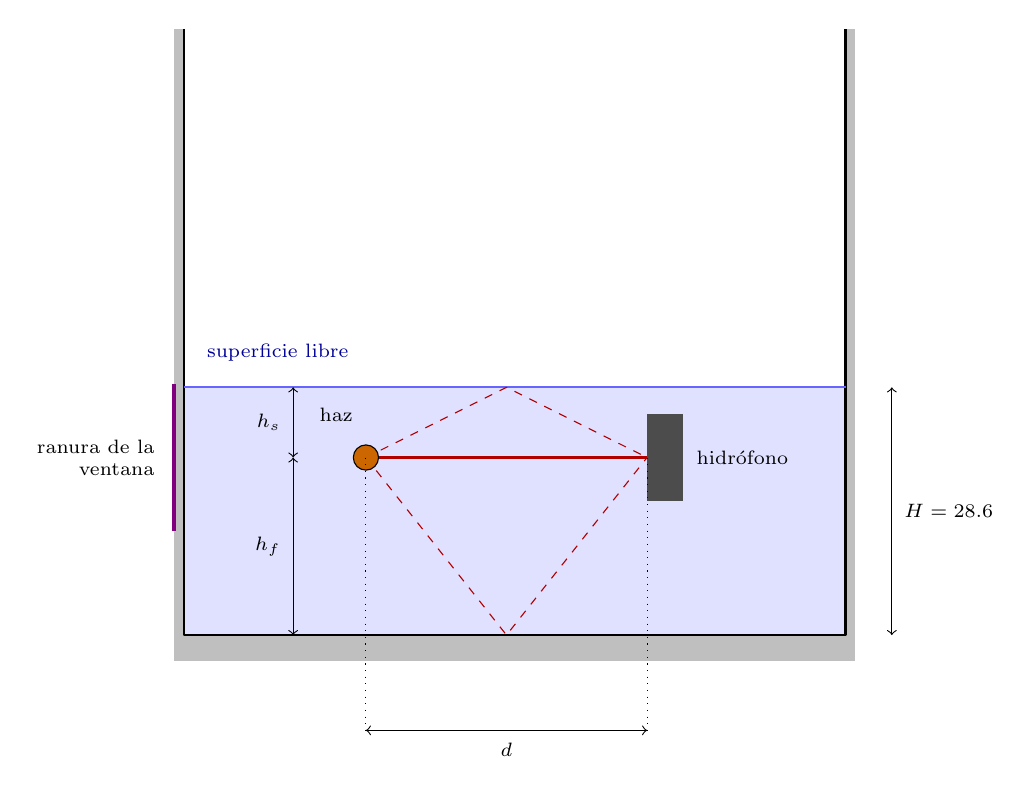
\begin{tikzpicture}[x=0.042cm, y=0.11cm, line join=round]

    % --- parámetros geométricos -----------------------------
    \def\Largo{200}      % longitud interna de la cavidad
    \def\Alto{70}        % altura interna de la cavidad
    \def\Espesor{3}      % espesor del acrílico
    \def\Tirante{28.6}   % tirante de líquido
    \def\Hhaz{20.5}      % altura del eje del haz sobre el fondo
    \def\Xhaz{55}        % posición del haz a lo largo de la celda
    \def\Dh{85}          % separación dibujada entre haz e hidrófono

    % --- líquido --------------------------------------------
    \fill[blue!12] (0,0) rectangle (\Largo,\Tirante);

    % --- paredes de acrílico --------------------------------
    \fill[black!25]
      (-\Espesor,-\Espesor) rectangle (0,\Alto);
    \fill[black!25]
      (\Largo,-\Espesor) rectangle (\Largo+\Espesor,\Alto);
    \fill[black!25]
      (-\Espesor,-\Espesor) rectangle (\Largo+\Espesor,0);

    % --- contorno de la cavidad -----------------------------
    \draw[thick] (0,\Alto) -- (0,0) -- (\Largo,0) -- (\Largo,\Alto);

    % --- superficie libre -----------------------------------
    \draw[blue!60, thick] (0,\Tirante) -- (\Largo,\Tirante);

    % --- trayectorias acústicas -----------------------------
    \draw[red!70!black, thick]
      (\Xhaz,\Hhaz) -- (\Xhaz+\Dh,\Hhaz);
    \draw[red!70!black, dashed]
      (\Xhaz,\Hhaz) -- (\Xhaz+0.5*\Dh,\Tirante)
                    -- (\Xhaz+\Dh,\Hhaz);
    \draw[red!70!black, dashed]
      (\Xhaz,\Hhaz) -- (\Xhaz+0.5*\Dh,0)
                    -- (\Xhaz+\Dh,\Hhaz);

    % --- haz visto de punta ---------------------------------
    \fill[orange!80!black] (\Xhaz,\Hhaz) circle (1.6mm);
    \draw (\Xhaz,\Hhaz) circle (1.6mm);

    % --- hidrófono ------------------------------------------
    \fill[black!70]
      (\Xhaz+\Dh,\Hhaz-5) rectangle (\Xhaz+\Dh+11,\Hhaz+5);

    % --- ranura de la ventana de cuarzo ---------------------
    \draw[violet, very thick] (-\Espesor,12) -- (-\Espesor,29);

    % --- cotas verticales -----------------------------------
    \draw[<->] (\Largo+14,0) -- (\Largo+14,\Tirante)
      node[midway, right=1pt] {\scriptsize $H = \SI{28.6}{\milli\meter}$};
    \draw[<->] (\Xhaz-22,0) -- (\Xhaz-22,\Hhaz)
      node[midway, left=1pt] {\scriptsize $h_f$};
    \draw[<->] (\Xhaz-22,\Hhaz) -- (\Xhaz-22,\Tirante)
      node[midway, left=1pt] {\scriptsize $h_s$};

    % --- cota horizontal ------------------------------------
    \draw[<->] (\Xhaz,-11) -- (\Xhaz+\Dh,-11)
      node[midway, below=1pt] {\scriptsize $d$};
    \draw[dotted] (\Xhaz,\Hhaz) -- (\Xhaz,-11);
    \draw[dotted] (\Xhaz+\Dh,\Hhaz) -- (\Xhaz+\Dh,-11);

    % --- rótulos --------------------------------------------
    \node[anchor=west, font=\scriptsize]
      at (\Xhaz+\Dh+12,\Hhaz) {hidrófono};
    \node[anchor=south, font=\scriptsize]
      at (\Xhaz-9,\Hhaz+3) {haz};
    \node[anchor=east, font=\scriptsize, align=right]
      at (-6,20.5) {ranura de la\\ventana};
    \node[anchor=west, font=\scriptsize, text=blue!60!black]
      at (4,\Tirante+4) {superficie libre};

  \end{tikzpicture}
  \caption{Corte de la celda en el plano que contiene al hidrófono. El
           haz se ve de punta, a la altura $h_f$ sobre el fondo que fija
           la ranura de la ventana de cuarzo. La separación $d$ entre el
           eje del haz y la cara sensora se mide en cada sesión. Las
           líneas punteadas son las trayectorias de las primeras
           reflexiones en la superficie libre y en el fondo. La escala vertical está
           exagerada respecto de la horizontal.}
  \label{fig:celda_corte}
\end{figure}


\section*{Posición del haz dentro de la cavidad}

La altura del haz sobre el fondo no es un parámetro libre: la fija la
ranura que aloja la ventana de cuarzo en la pared larga, que abarca de
\SI{12}{\milli\meter} a \SI{29}{\milli\meter} medidos desde el fondo.
El haz atraviesa el centro de esa ranura, de modo que su altura sobre
el fondo es

\begin{equation}
    h_f = \frac{\SI{12}{\milli\meter} + \SI{29}{\milli\meter}}{2}
        = \SI{20.5}{\milli\meter}.
    \label{eq:altura_haz}
\end{equation}

La distancia del haz a la superficie libre se obtiene restando esa
altura al tirante de líquido establecido en la \cref{eq:tirante}:

\begin{equation}
    h_s = H - h_f = \SI{28.6}{\milli\meter} - \SI{20.5}{\milli\meter}
        = \SI{8.1}{\milli\meter}.
    \label{eq:altura_superficie}
\end{equation}

Conviene notar que $h_s$ depende del volumen vertido y $h_f$ no. El
llenado desplaza la superficie libre; la ventana de cuarzo permanece
donde está.

\section*{Trayectorias}

Con la fuente lineal a distancia $d$ del hidrófono y a alturas $h_s$ y
$h_f$ de las fronteras horizontales, las longitudes de las
trayectorias son las siguientes.

La señal directa recorre la distancia que separa la columna iluminada
del transductor:

\begin{equation}
    \ell_{\text{dir}} = d.
    \label{eq:traj_directa}
\end{equation}

La reflexión en la superficie libre se construye colocando una fuente
imagen a una altura $h_s$ por encima de la superficie, es decir, a
$2h_s$ de la fuente real. La trayectoria es la hipotenusa del triángulo
rectángulo cuyos catetos son $d$ y $2h_s$:

\begin{equation}
    \ell_{\text{sup}} = \sqrt{d^{2} + (2h_s)^{2}}.
    \label{eq:traj_superficie}
\end{equation}

La reflexión en el fondo se obtiene de forma análoga con la fuente
imagen a $2h_f$:

\begin{equation}
    \ell_{\text{fondo}} = \sqrt{d^{2} + (2h_f)^{2}}.
    \label{eq:traj_fondo}
\end{equation}

Las reflexiones en las paredes transversales de la celda ocurren a una
distancia del orden de la mitad de la longitud interna de la cavidad,
aproximadamente \SI{100}{\milli\meter}. Su arribo es tan posterior al
de las anteriores que basta acotarlo: no compite con la ventana útil,
pero sí fija el límite superior de la longitud de registro que tiene
sentido conservar.

El tiempo de arribo de cada trayectoria es su longitud dividida entre
la velocidad del sonido:

\begin{equation}
    t = \frac{\ell}{v}.
    \label{eq:tiempo_arribo}
\end{equation}

\section*{Evaluación para la geometría nominal}

Tomando el valor nominal $d = \SI{10}{\milli\meter}$ reportado por
Rangel Mendieta \cite{Rangel2023}, junto con
$h_f = \SI{20.5}{\milli\meter}$, $h_s = \SI{8.1}{\milli\meter}$ y
$v = \SI{1480}{\meter\per\second}$, las
\crefrange{eq:traj_directa}{eq:tiempo_arribo} producen los valores de
la \cref{tab:tiempos_celda}: \SI{10.0}{\milli\meter} y
\SI{6.8}{\micro\second} para la señal directa,
\SI{19.0}{\milli\meter} y \SI{12.9}{\micro\second} para la reflexión
en la superficie libre, \SI{42.1}{\milli\meter} y
\SI{28.5}{\micro\second} para la reflexión en el fondo, y
aproximadamente \SI{100}{\milli\meter} y \SI{67.6}{\micro\second} para
las paredes transversales.

La ventana temporal libre de reflexiones es la diferencia entre los dos
primeros arribos:

\begin{equation}
    \Delta t = \frac{\sqrt{d^{2} + (2h_s)^{2}} - d}{v}
             \approx \SI{6.1}{\micro\second}.
    \label{eq:ventana_util}
\end{equation}

\section*{Dependencia respecto del montaje}

El láser es un recurso compartido y la celda no se encuentra fijada de
manera permanente a la mesa óptica, de modo que la geometría del
arreglo se restablece al inicio de cada sesión. En consecuencia, $d$ no
es una constante del sistema sino un parámetro del montaje del día, y
los valores anteriores corresponden a la geometría nominal, no a una
propiedad invariante de la celda.

La \cref{eq:ventana_util} muestra que la ventana útil se acorta al
aumentar $d$. Con el hidrófono a \SI{5}{\milli\meter} del haz la
ventana se extiende a aproximadamente \SI{8.1}{\micro\second}; a
\SI{15}{\milli\meter} se reduce a cerca de \SI{4.8}{\micro\second}. La
diferencia no es despreciable frente a la duración del pulso bipolar
que se pretende resolver, por lo que la base de tiempo y la longitud de
registro configuradas en el osciloscopio deben verificarse contra la
geometría efectiva de cada sesión y no darse por heredadas.

El procedimiento para hacerlo consta de tres pasos. Primero, medir con
vernier la separación entre la cara sensora del hidrófono y el eje del
haz, lo que proporciona $d$. Segundo, confirmar el volumen vertido, que
mediante la \cref{eq:tirante} determina el tirante $H$ y con él la
altura $h_s$ de la \cref{eq:altura_superficie}; la altura $h_f$ no
requiere verificación, pues la fija la ranura de la ventana de cuarzo.
Tercero, evaluar la \cref{eq:ventana_util} con esos valores y comparar
el resultado con la base de tiempo configurada.

Ninguna de estas dos magnitudes se registra actualmente en los
metadatos de sesión. Su incorporación al formato descrito en la
\cref{sec:formato_datos} se plantea en el \cref{cap:conclusiones} como
mejora pendiente: mientras no se registren, la reconstrucción posterior
de la ventana útil de una sesión depende de la bitácora del operador y
no del archivo de datos.
